\title{INTD262: Aztec Species Classification in Mesoamerica}
\author{Dr. Jordan Hanson - Whittier College Dept. of Physics and Astronomy}
\date{\today}
\documentclass[12pt]{article}
\usepackage[margin=1.5cm]{geometry}
\usepackage{hyperref}
\usepackage{graphicx}
\usepackage{amsmath}
\begin{document}
\maketitle

\section{Introduction}

In this activity, we will compare and contrast the Linnaean and modern species classification with what appears to be a species classification system from the Aztecs from chapter 1 of \textit{Science in Latin America}.  First, we will review, from an evolutionary perspective, why species classification makes sense.  Second, we will review a modern scientific publication \cite{10.1016/j.cub.2014.03.016}

\section{Classification of Species}

\begin{figure}[h]
\centering
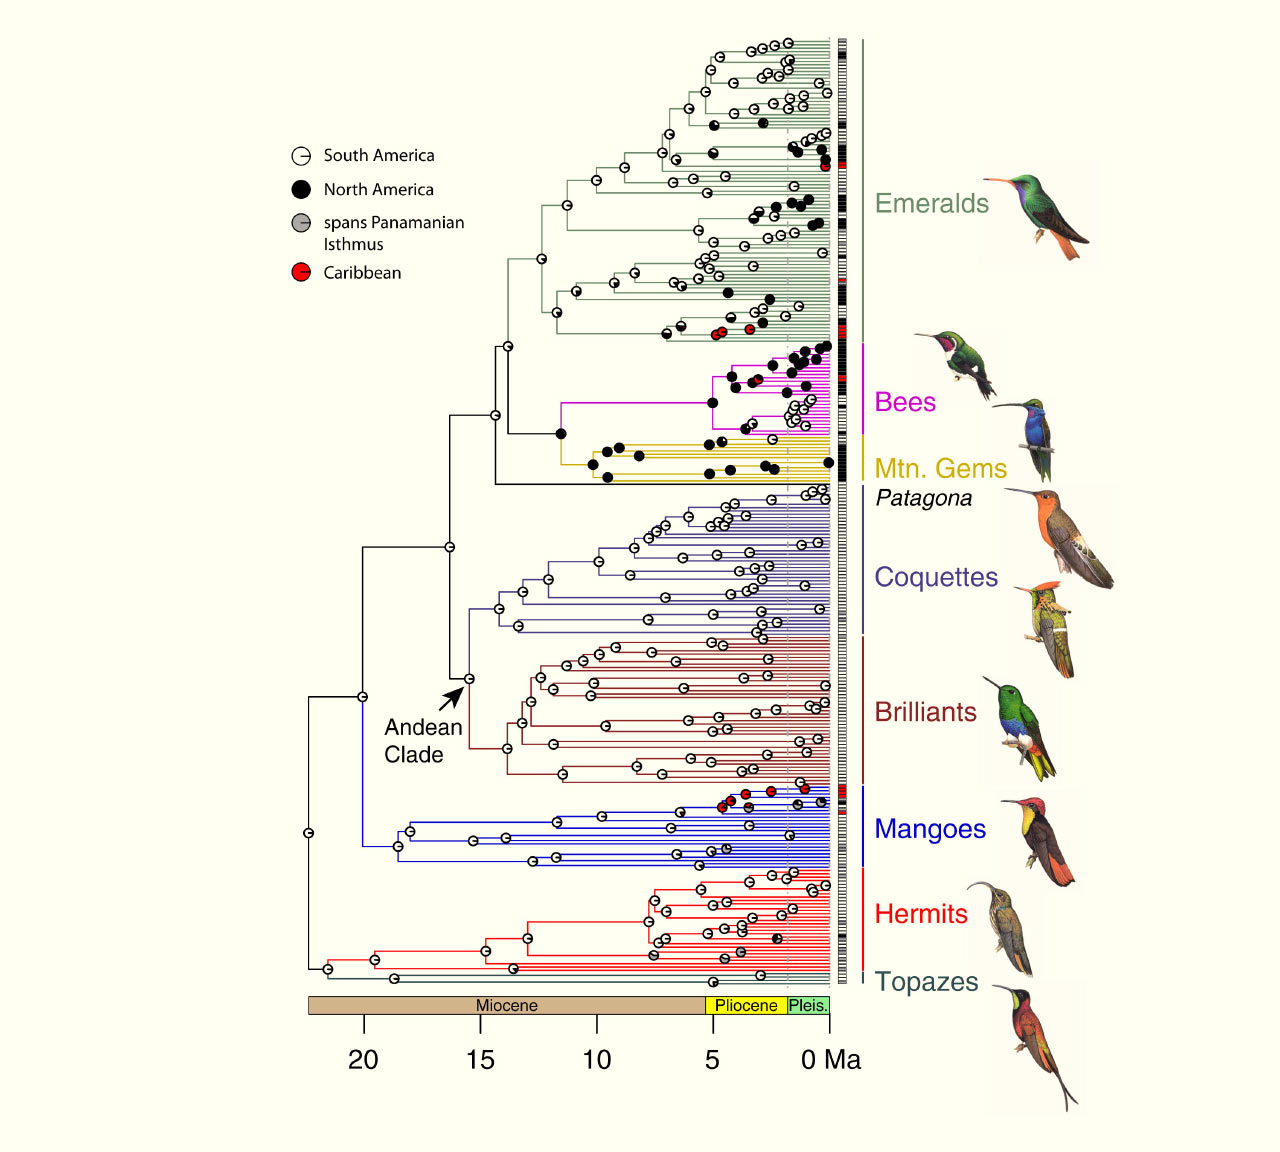
\includegraphics[width=0.75\textwidth]{figures/hummingbird.jpg}
\caption{\label{fig:1} In a recent publication, the }
\end{figure}

\begin{itemize}
\item \textit{quetzal huitzilin}
\item \textit{xi huitzilin}
\item \textit{chalchi huitzilin}
\item \textit{yiauhtic huitzilin}
\item \textit{tlapal huitzilin}
\item \textit{aiopal huitzilin}
\item \textit{tle huitzilin}
\item \textit{quapa huitzilin}
\end{itemize}

\section{Conclusion}

Our goal is to develop a nuanced understanding of the demarcation between fields.  Our individual versions of Fig. \ref{fig:1} will depend on our perspective.  Our individual versions, however, should be correlated.

\begin{figure}[hb]
\centering
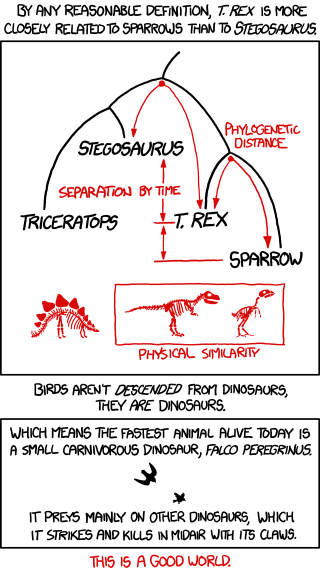
\includegraphics[width=0.25\textwidth]{figures/birds_and_dinosaurs.png}
\caption{\label{fig:2} Phylogenetic distance quantifies the evolutionary relationship between species ... \textit{even dinosaurs!} (Credit: \url{xkcd.com}).}
\end{figure}

\bibliographystyle{plain}
\bibliography{biblio_1}

\end{document}
